\chapter{Simulations of the Artificial SMMF}\label{app:SMMF_sims}


\section{Model}

The artificial data used in the simulations of the \gls{smmf} were created using two very simplistic models, either separately or in combination, which were physically motivated by sunspots and \glspl{ar} on the solar surface \citep{van_driel-gesztelyi_evolution_2015}:

\begin{enumerate}
	
	\item{{\bf Cosine}: in this model a source was simulated as a single region which ingresses the visible disk from one limb, traverses across the disk, before egressing the other limb (see Fig.~\ref{fig:cosine_model}). The physical motivation for this would be a single, concentrated source of imbalanced magnetic flux at the photospheric level. This method induces no sign change of the simulated source; it remains the same polarity always. This was simulated as a rectified sinusoidal signal, with a 50$\%$ duty cycle (i.e. it is only visible during times on near-side of the disk).}
	
	\item{{\bf Sign change}: in this model a source was simulated as two regions of opposite polarity, such as sunspot pairs or a \gls{bmr}. The leading region contributes more at the start of the transit during ingress, and the trailing source contributes more at the end of the transit during egress; hence at the middle of the transit we assume there is a sign change in the overall signal, see Fig.~\ref{fig:sgn_cng_model}. This was simulated as a rectified sinusoidal signal, and was multiplied by a cosinusoidal signal of the same period to provide the projection of the pair of regions. This operation results in a rectified sinusoidal signal with half the period.}
	
\end{enumerate}

\begin{figure}
	\centering
	\subfloat[`cosine' model \label{fig:cosine_model}]{
\includegraphics[width=0.35\columnwidth]{cosine_model.pdf}} 
	\qquad
	\subfloat[`sign change' model \label{fig:sgn_cng_model}]{
\includegraphics[width=0.35\columnwidth]{sgn_cng_model.pdf}}
	\caption{Schematic representations of the two models of the artificial SMMF. (a) shows the cosine model with a single source of constant polarity transiting the visible disk. (b) shown the sign change model whereby there are 2 regions of opposite polarity transiting the disk, and their contribution to the SMMF changes during the transit.}  \label{fig:artificial_models}
\end{figure}


There were several variables that allowed us to change the physics of the simulations. These were:

\begin{itemize}
	\item{{\bf $N$}: Number of sources}
	\item{{\bf $t_0$}: Start time of source appearance}
	\item{{\bf $A$}: Amplitude of sources}
	\item{{\bf $\lambda$}: Latitude of sources}
	\item{{\bf $\tau$}: Decay time of sources}
	\item{{\bf $\phi$}: Additional phase of sources}
\end{itemize}

Using these variables, the mathematical forms of the two model types for a single source are expressed by equation~(\ref{eq:cosine_model}) and equation~(\ref{eq:sgn_cng_model}). In these equations $t' = t - t_0$, $\Pi_{P/2}(t)$ is a window function to define the transit period of the simulated source on the visible side of the solar disk, $\mathrm{III}_{P}$ is a Dirac comb of repetition period, P, and $\Pi_{T}(t)$ is a window function defining the total observation period:

\begin{equation}
B_{\mathrm{cosine}}(t) = \left[ A e^{-t'/\tau} \, \left( \cos{\left(\frac{2\pi}{P}t' + \phi\right)} \, \Pi_{P/2}(t) \right) * \mathrm{III}_{P} \right] \times \Pi_{T}(t) \, ;
\label{eq:cosine_model}
\end{equation}


\begin{equation}
B_{\mathrm{sign-change}}(t) = \left[ A e^{-t'/\tau} \, \left( \cos{\left(\frac{2\pi}{P}t' + \phi\right)} \, \sin{\left(\frac{2\pi}{P}t' + \phi\right)} \, \Pi_{P/2}(t) \right) * \mathrm{III}_{P} \right] \times \Pi_{T}(t) \, .
\label{eq:sgn_cng_model}
\end{equation}

The time series of a single modelled source for each model is shown in Figure~\ref{fig:artificial_models}.

\begin{figure}[ht!]
	\centering
	\subfloat[`cosine' model \label{fig:cosine_TS}]{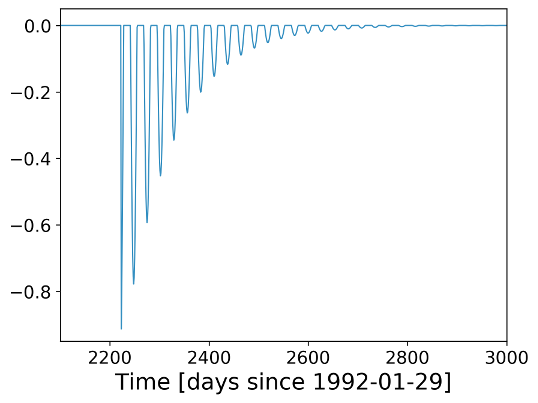
\includegraphics[width=0.45\columnwidth]{fake_TS_cosine_rescaled.png}} 
	\qquad
	\subfloat[`sign change' model \label{fig:sgn_cng_TS}]{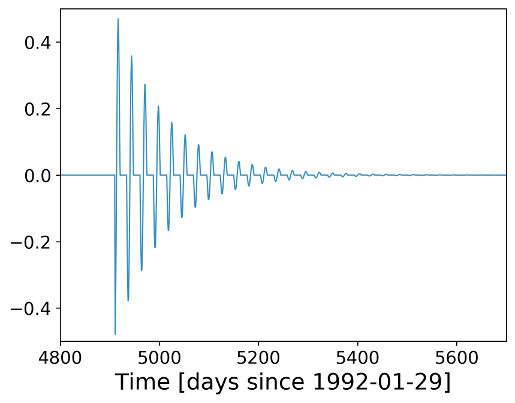
\includegraphics[width=0.45\columnwidth]{fake_TS_sgn_cng_rescaled.png}}
	\caption{A single realisation of (a) the cosine model, and (b) the sign change model.}  
	\label{fig:artificial_TS}
\end{figure}


\section{Configuration of the Simulations}

A flowchart describing the steps in the simulations is shown in Figure~\ref{fig:flowchart}. The simulations require the user to select the number of sources to be modelled. Using this information, the user selects whether to draw N seed/start times ($t_0$) from either a \gls{kde} of the \gls{ssn}, or from a uniform distribution between the start and end times. The former will give an output which is more physical, but the latter is useful for testing.


\begin{figure}[ht!]
	\centering
	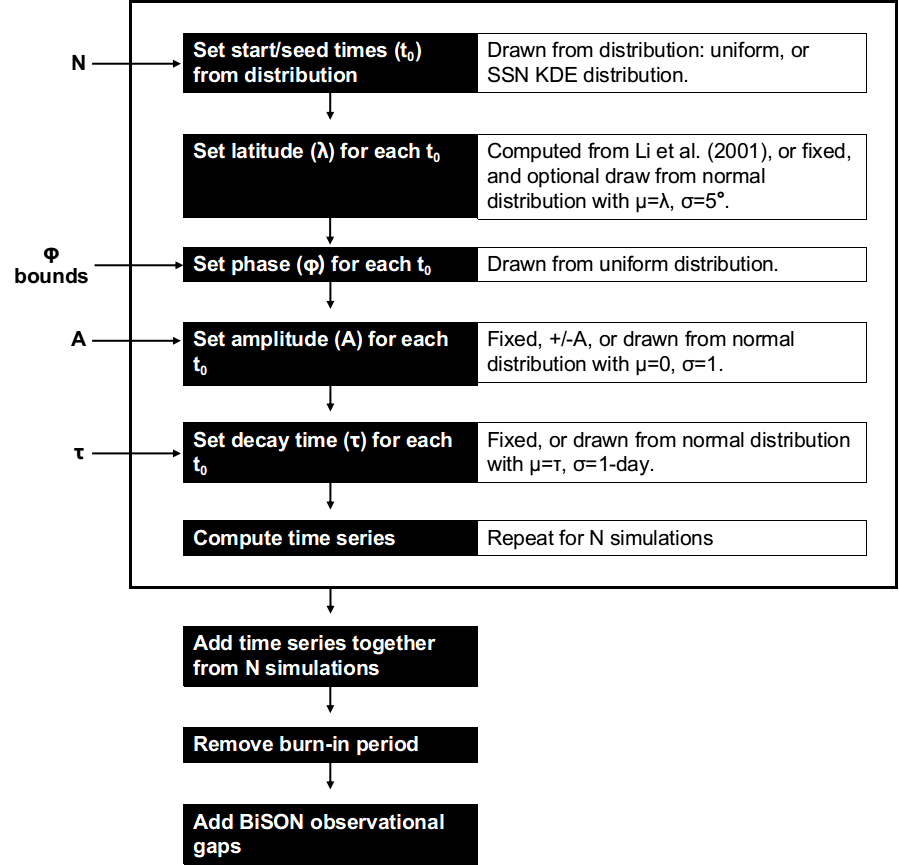
\includegraphics[width=0.85\columnwidth]{flow_chart_2.png}
	\caption{Flowchart showing the step-by-step processes in the generation of the artificial SMMF time series data.}
	\label{fig:flowchart}
\end{figure}


From the generated seed times, latitudes are computed using a model for the migration of spots during the Solar Cycle \citep{li_latitude_2001}, and the differential rotation frequency at that latitude is taken from a model of the solar differential rotation \citep{snodgrass_magnetic_1983}. 

Values are then assigned for the phase, amplitude, and decay time of each source (the user can set these parameters, or it is also possible to randomly draw them from a distribution). Each individual source is simulated according to equation~(\ref{eq:cosine_model}) or equation~(\ref{eq:sgn_cng_model}). Following the simulation of N sources, the full time-series is computed by adding all N source contributions together. Finally, a burn-in period is removed, which allows the artificial \gls{smmf} to settle prior to the start of `observations', and then we can inject gaps into the artificial time series which are concurrent with the gaps in the \gls{bison} observations.

The aim of creating artificial data was to produce a representative power spectrum to that of the \gls{bison} \gls{smmf}. We assumed that the sources of the \gls{smmf} are \glspl{ar} and \glspl{mfc}, therefore we aimed to produce a time series that physically represented these sources, i.e. comparable to the sunspot number. To do this we produced an average number of sources on the visible disk during the maximum of cycle 23 close to the sunspot number. At solar maximum during cycle 23, the number of daily spots on the disk is around 150 -- 200. 

\begin{figure}[!ht]
	\centering
	\subfloat[Burn-in]{
		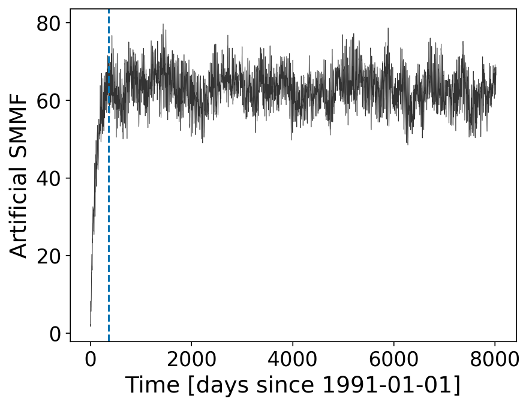
\includegraphics[width=0.45\columnwidth]{burn-in_TS_rescaled.png}
		\label{fig:artificial_sim_burn-in}}
	\qquad
	\subfloat[Number of sources in the simulation after burn-in]{
		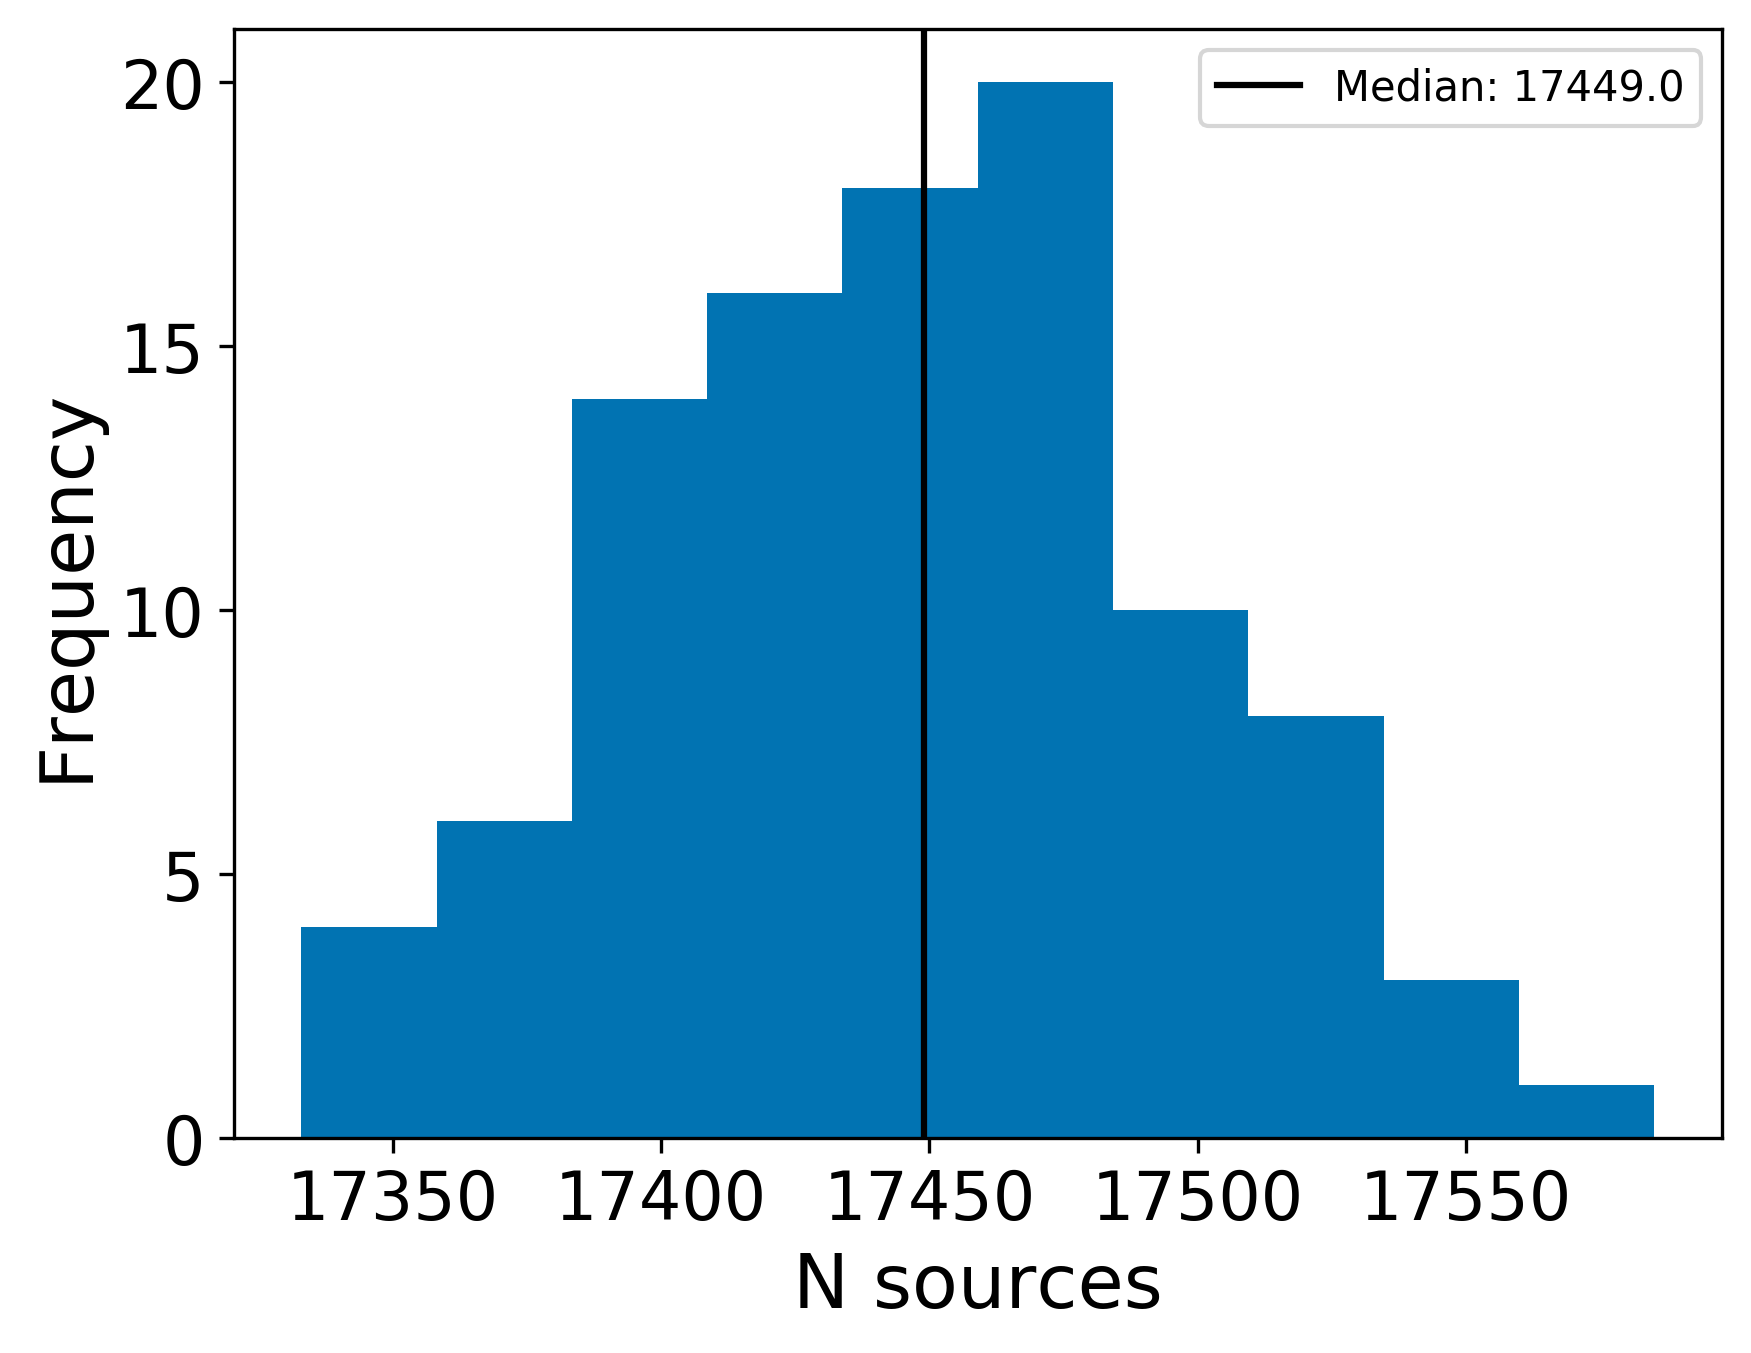
\includegraphics[width=0.45\columnwidth]{N_hist.png}
		\label{fig:artificial_sim_N}} \\
	
	\qquad
	
	\subfloat[Sources on the visible disk]{
		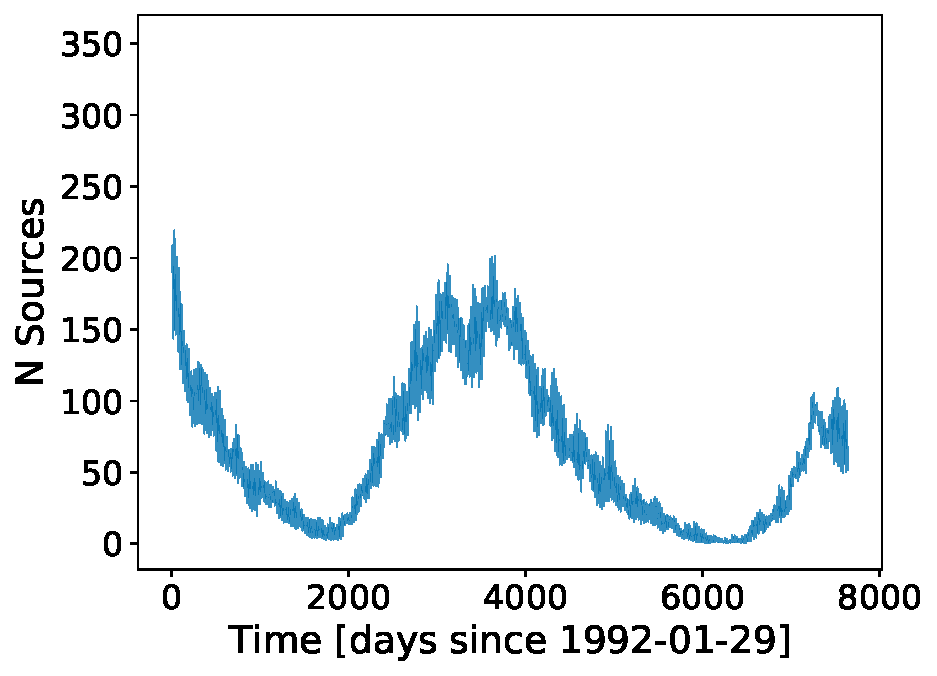
\includegraphics[width=0.45\columnwidth]{Fake_sources.pdf}
		\label{fig:artificial_sim_sources}}
	\qquad
	\subfloat[Sunspot number]{
		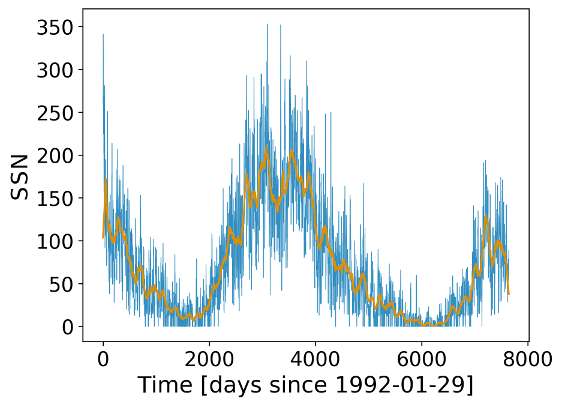
\includegraphics[width=0.45\columnwidth]{SSN_rescaled.png}
		\label{fig:artificial_sim_SSN}}
	
	\caption{(a) the burn-in period required to ensure that the interference of sources stabilises. The dashed-vertical line marks one year, showing the sources have stabilised. (b) histogram of the number of sources which remain in the simulation, after the burn-in is removed. (c) the number of simulated sources on the visible disk over the BiSON observational epoch. (d) the daily-averaged sunspot number (blue, and the monthly-averaged sunspot number (orange)).}
	\label{fig:artificial_sim_config}
\end{figure}


We included $\sim$1--year for burn-in, to allow the interferences between the sources stabilises (see Figure~\ref{fig:artificial_sim_burn-in}). After a year the number of sources on the visible disk has stabilised, providing a stable \gls{smmf}, hence a burn-in period from 01/01/1991 -- 29/01/1992 is sufficient. With this burn-in period, we chose to select N~=~20000 and $\tau$~=~100 days, which produces a median total of $\sim$17450 sources over the \gls{bison} observational epoch of 7633 days, with an average of around 100 -- 200 sources per day on the visible disk during solar cycle 23 maximum, as shown in Figure~\ref{fig:artificial_sim_config}.




\section{Outputs}


The simulation produces a time series output from the combination of all the sources with and without the inclusion of \gls{bison} observational gaps, along with the Fourier transforms of both. 

For quality assurance, a butterfly diagram is also generated per simulation to understand whether the simulation is representative of the Sun's \glspl{ar}. A butterfly diagram, from a realisation which allows for a more realistic, stochastic simulation whereby the values for parameters are drawn from a distribution with scatter, is shown in Figure~\ref{fig:fake_butterfly}. This butterfly diagram shows a strong resemblance to a true, observational butterfly diagram of the Sun. This provides us with confidence that the simulations are well-representing \glspl{ar} on the solar disk.


\begin{figure}[ht!]
	\centering
	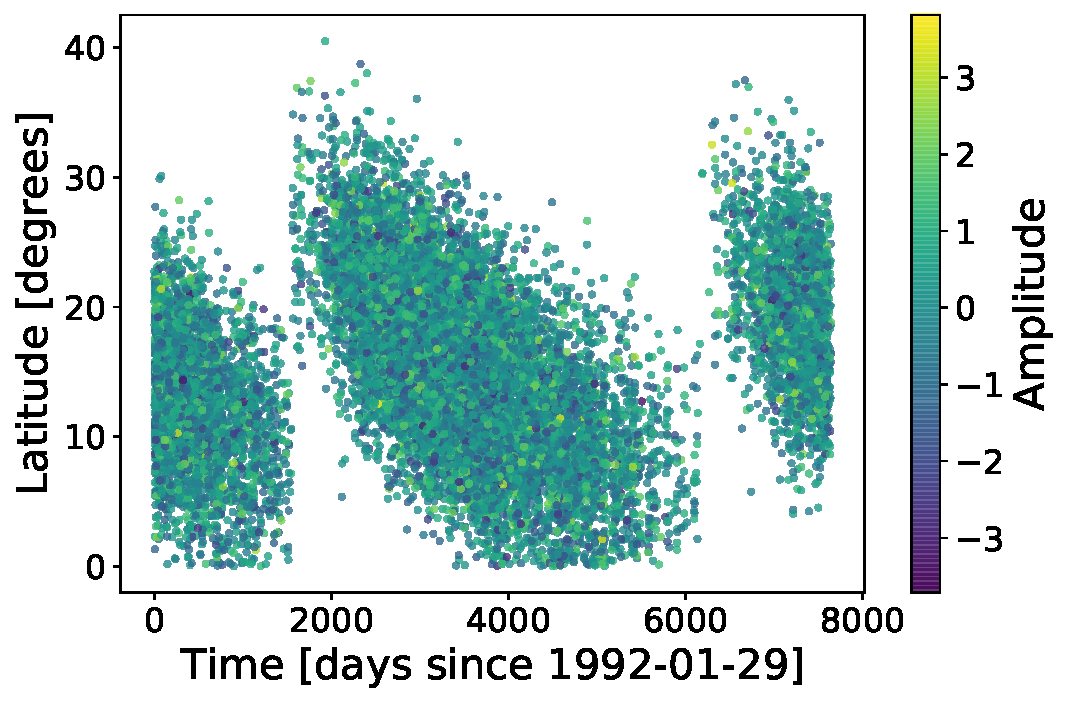
\includegraphics[width=0.85\columnwidth]{24h_fake_butterfly.pdf}
	\caption{Artificial butterfly diagram generated from the simulations, allowing for the parameters to be drawn from distributions, to add stochasticity into the simulation.}
	\label{fig:fake_butterfly}
\end{figure}


The resultant power spectra for the two different models (`cosine' and `sign change') show different features, which can be seen in the limit spectra shown in Figure~\ref{fig:artificial_LS}. These limit spectra were made by combining 100 realisations of the power spectrum. Each individual power spectrum was made using only a single source starting at $t_0 = 0$, and allowing only the phase to vary between the different realisations.

\begin{figure}[ht!]
	\centering
	\subfloat[`cosine' model \label{fig:cosine_LS}]{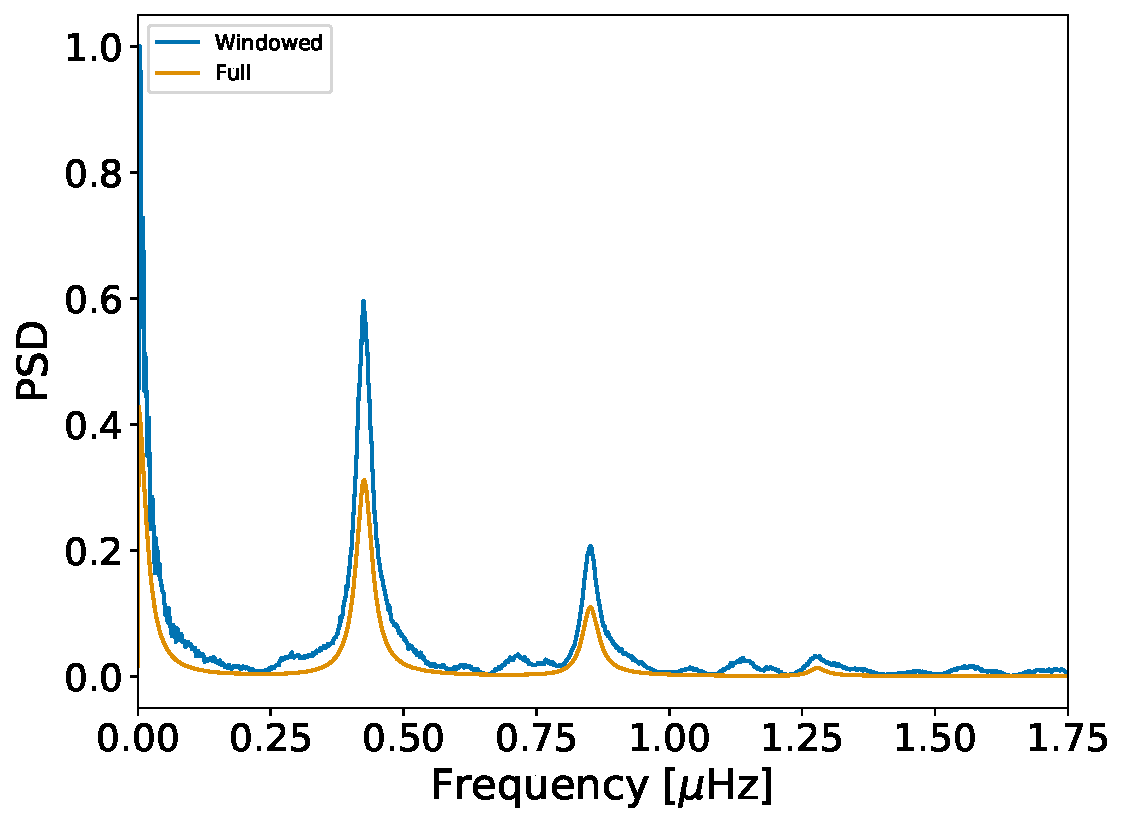
\includegraphics[width=0.45\columnwidth]{cosine_LS.pdf}} 
	\qquad
	\subfloat[`sign change' model \label{fig:sgn_cng_LS}]{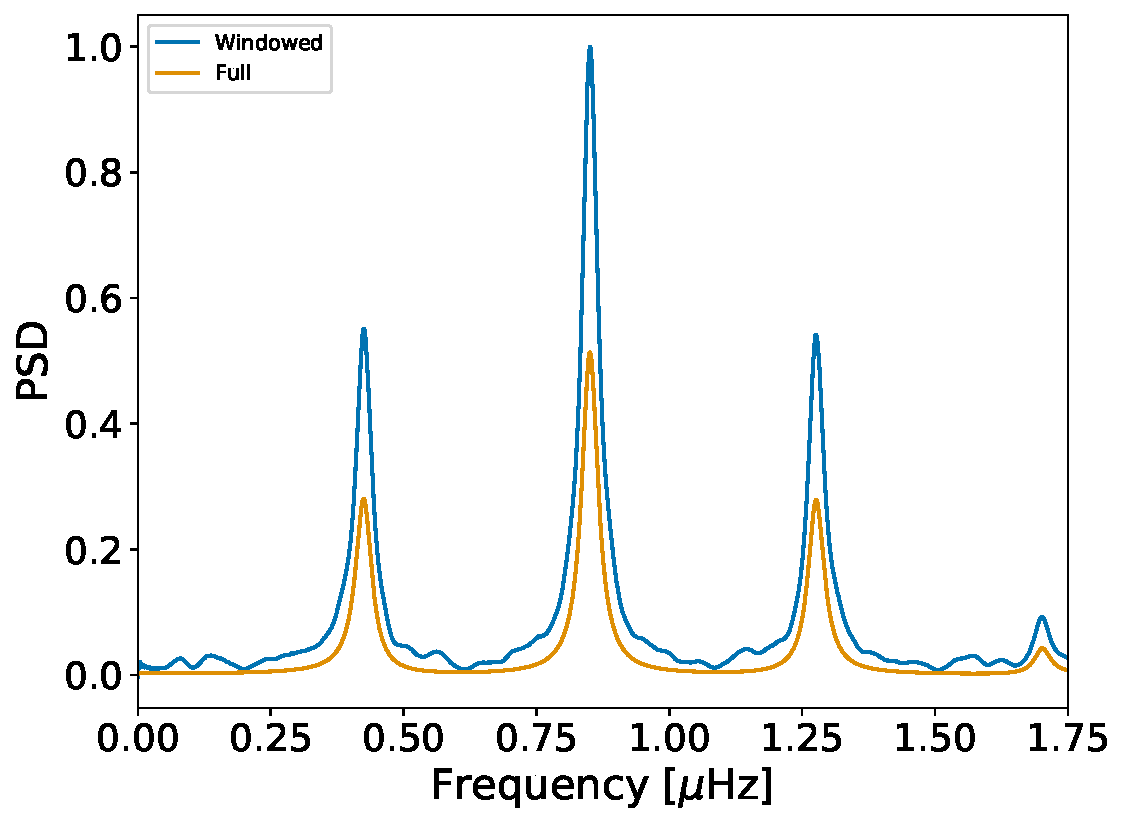
\includegraphics[width=0.45\columnwidth]{sgn_cng_LS.pdf}}
	\caption{Limit spectrum from 100 realisations of the cosine model (a) and the sign change model (b) using a single source in each model.}  \label{fig:artificial_LS}
\end{figure}

It is clear that the `cosine' model produces a strong peak at the rotational period in the simulation, and a harmonic peak at twice that frequency. This model also produces a significant amount of power at low frequency due to the non-zero mean of the simulated time series. 

On the other hand, the `sign change' model has near-zero low frequency power due to the $\sim$zero mean of the time series. The `sign change' model also produces a strong peak at half the period of rotation in the simulation. There is a smaller, yet strong peak at the rotational period and at a harmonic of the rotation of 3 times the period. In addition to the limit spectra, we show in Figure~\ref{fig:artificial_sim_outs} the time series and power spectra for individual realisations of the simulations.


\begin{figure}[!ht]
	\centering
	\subfloat[Cosine model time series]{
		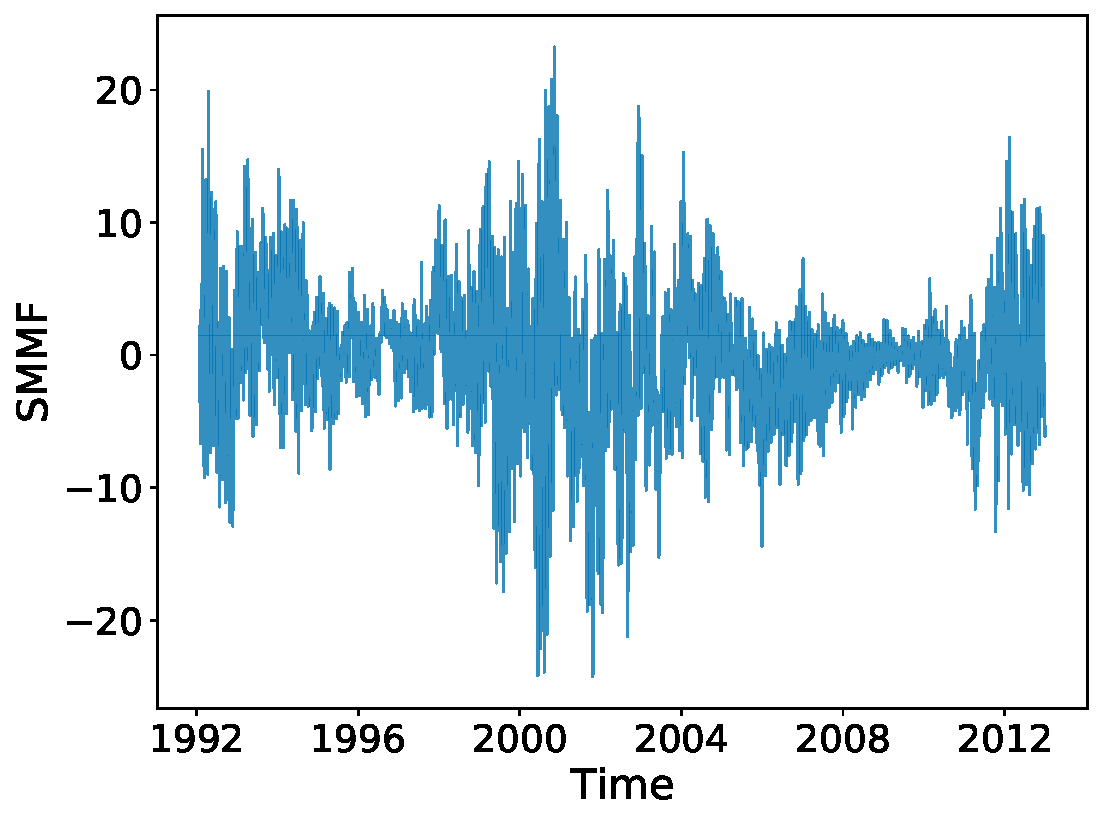
\includegraphics[width=0.45\columnwidth]{cosine_single_TS.pdf}
		\label{fig:csn_model_TS}}
	\qquad
	\subfloat[Cosine model power spectrum]{
		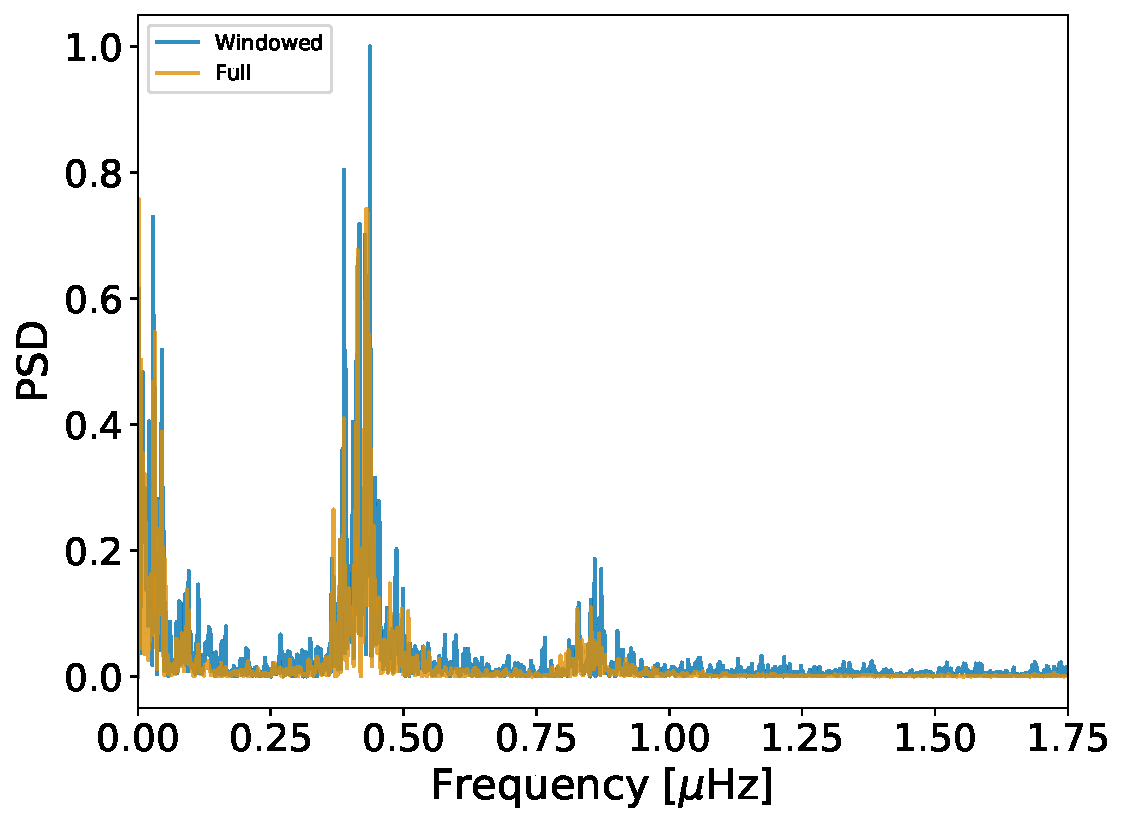
\includegraphics[width=0.45\columnwidth]{cosine_single_spectrum.pdf}
		\label{fig:csn_model_FT}} \\
	
	\qquad
	
	\subfloat[Sign change model time series]{
		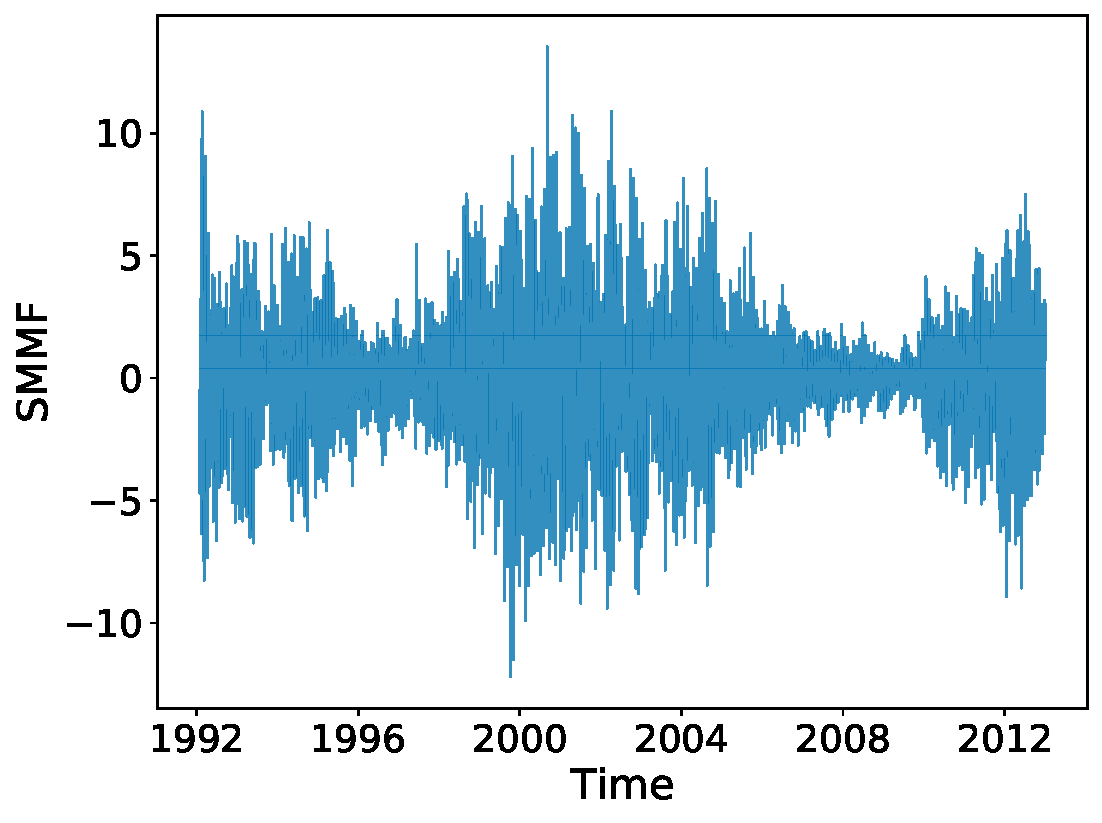
\includegraphics[width=0.45\columnwidth]{sgn_cng_single_TS.pdf}
		\label{fig:sc_model_TS}}
	\qquad
	\subfloat[Sign change model power spectrum]{
		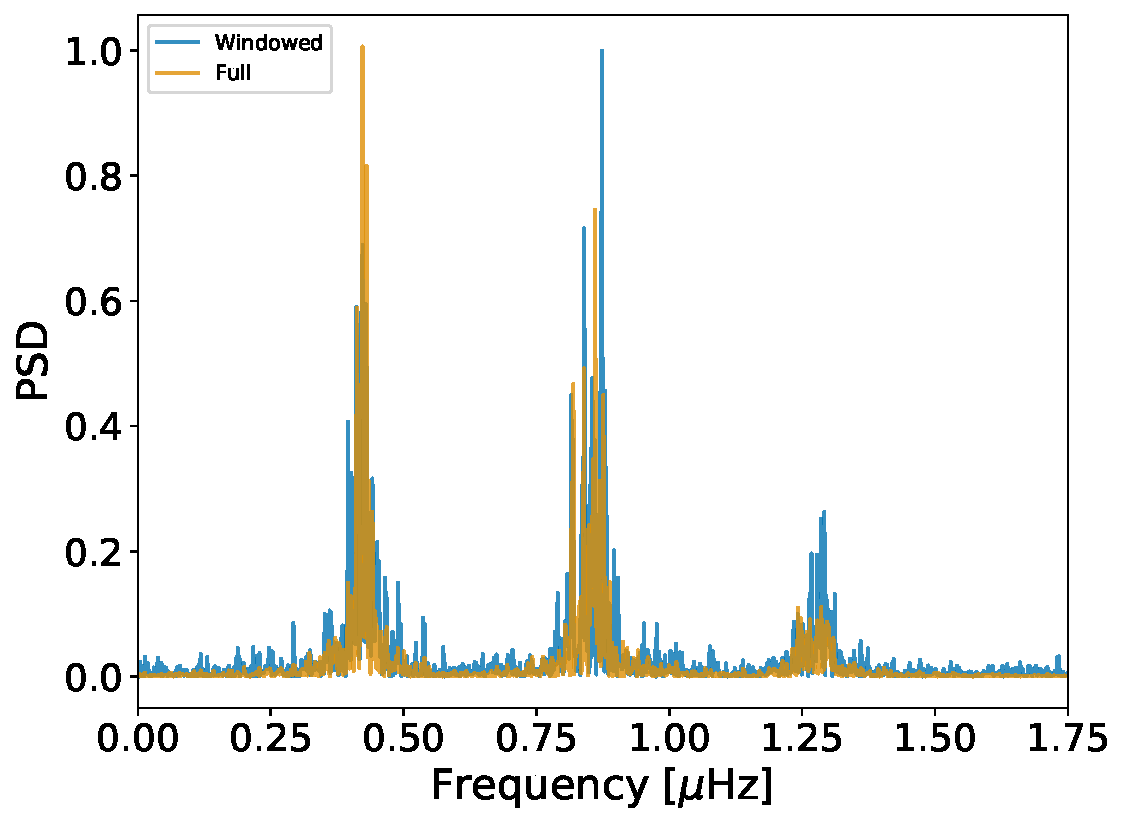
\includegraphics[width=0.45\columnwidth]{sgn_cng_single_spectrum.pdf}
		\label{fig:sc_model_FT}}
	
	\caption{Time series and power spectra for realisations of the simulations using the cosine and sign change models.}
	\label{fig:artificial_sim_outs}
\end{figure}

These realisations show the simulated \gls{smmf} on a daily cadence. The plots show the stark difference in the time series produced by each model. There are many deviations from a zero mean in the `cosine' model case, which clearly demonstrates the origin of the low frequency power. In the `sign change' model realisation, the data show a compelling near--zero mean, hence the origin of the near--zero low frequency power in the spectrum.

Both realisations of the simulations result in a time series which does resemble some of the features of the \gls{bison} \gls{smmf} observations, and hence there is a justification for using both in combination to simulate a representative model of the \gls{smmf}. This is supported also by the power spectra for each realisation, and the limit spectra. The power spectrum of the \gls{bison} \gls{smmf} shows a strong harmonic peak at three times the period, which is more prominent in the `sign change' model than the `cosine'. The `sign change' model power spectrum also shows a similar splitting around the half--period frequency, resembling that of the \gls{bison} spectrum in Figure~\ref{fig:BiSON_vs_WSO_PSDs}.
